%%%%%%%%%%%%%%%%%%%%%%%%%%%%%%%%%%%%%%%%%
% Lachaise Assignment
% LaTeX Template
% Version 1.0 (26/6/2018)
%
% This template originates from:
% http://www.LaTeXTemplates.com
%
% Authors:
% Marion Lachaise & François Févotte
% Vel (vel@LaTeXTemplates.com)
%
% License:
% CC BY-NC-SA 3.0 (http://creativecommons.org/licenses/by-nc-sa/3.0/)
% 
%%%%%%%%%%%%%%%%%%%%%%%%%%%%%%%%%%%%%%%%%

%----------------------------------------------------------------------------------------
%	PACKAGES AND OTHER DOCUMENT CONFIGURATIONS
%----------------------------------------------------------------------------------------

\documentclass[12pt,a4paper,oneside]{article}

\usepackage[utf8]{inputenc}
\usepackage[russian]{babel}
\usepackage{graphicx}
\usepackage{wrapfig}
\usepackage{float}
\usepackage{subcaption}
\usepackage{xcolor}
\definecolor{mygray}{gray}{0.4}
\usepackage[top=2.5cm,bottom=2.5cm,right=2.5cm,left=2.5cm,bindingoffset=0cm]{geometry}
\usepackage[colorlinks=true, a4paper=true, pdfstartview=FitV,
linkcolor=black, citecolor=mygray, urlcolor=mygray]{hyperref}
% \usepackage{natbib}


%%%%%%%%%%%%%%%%%%%%%%%%%%%%%%%%%%%%%%%%%
% Lachaise Assignment
% Structure Specification File
% Version 1.0 (26/6/2018)
%
% This template originates from:
% http://www.LaTeXTemplates.com
%
% Authors:
% Marion Lachaise & François Févotte
% Vel (vel@LaTeXTemplates.com)
%
% License:
% CC BY-NC-SA 3.0 (http://creativecommons.org/licenses/by-nc-sa/3.0/)
% 
%%%%%%%%%%%%%%%%%%%%%%%%%%%%%%%%%%%%%%%%%

%----------------------------------------------------------------------------------------
%	PACKAGES AND OTHER DOCUMENT CONFIGURATIONS
%----------------------------------------------------------------------------------------

\usepackage{amsmath,amsfonts,stmaryrd,amssymb} % Math packages

\usepackage{enumerate} % Custom item numbers for enumerations

\usepackage[ruled]{algorithm2e} % Algorithms

\usepackage[framemethod=tikz]{mdframed} % Allows defining custom boxed/framed environments

\usepackage{listings} % File listings, with syntax highlighting
\lstset{
	basicstyle=\ttfamily, % Typeset listings in monospace font
}

%----------------------------------------------------------------------------------------
%	DOCUMENT MARGINS
%----------------------------------------------------------------------------------------

\usepackage{geometry} % Required for adjusting page dimensions and margins

\geometry{
	paper=a4paper, % Paper size, change to letterpaper for US letter size
	top=2.5cm, % Top margin
	bottom=3cm, % Bottom margin
	left=2.5cm, % Left margin
	right=2.5cm, % Right margin
	headheight=14pt, % Header height
	footskip=1.5cm, % Space from the bottom margin to the baseline of the footer
	headsep=1.2cm, % Space from the top margin to the baseline of the header
	%showframe, % Uncomment to show how the type block is set on the page
}

%----------------------------------------------------------------------------------------
%	FONTS
%----------------------------------------------------------------------------------------

\usepackage[utf8]{inputenc} % Required for inputting international characters
\usepackage[T1]{fontenc} % Output font encoding for international characters

\usepackage{XCharter} % Use the XCharter fonts

%----------------------------------------------------------------------------------------
%	COMMAND LINE ENVIRONMENT
%----------------------------------------------------------------------------------------

% Usage:
% \begin{commandline}
%	\begin{verbatim}
%		$ ls
%		
%		Applications	Desktop	...
%	\end{verbatim}
% \end{commandline}

\mdfdefinestyle{commandline}{
	leftmargin=10pt,
	rightmargin=10pt,
	innerleftmargin=15pt,
	middlelinecolor=black!50!white,
	middlelinewidth=2pt,
	frametitlerule=false,
	backgroundcolor=black!5!white,
	frametitle={Command Line},
	frametitlefont={\normalfont\sffamily\color{white}\hspace{-1em}},
	frametitlebackgroundcolor=black!50!white,
	nobreak,
}

% Define a custom environment for command-line snapshots
\newenvironment{commandline}{
	\medskip
	\begin{mdframed}[style=commandline]
}{
	\end{mdframed}
	\medskip
}

%----------------------------------------------------------------------------------------
%	FILE CONTENTS ENVIRONMENT
%----------------------------------------------------------------------------------------

% Usage:
% \begin{file}[optional filename, defaults to "File"]
%	File contents, for example, with a listings environment
% \end{file}

\mdfdefinestyle{file}{
	innertopmargin=1.6\baselineskip,
	innerbottommargin=0.8\baselineskip,
	topline=false, bottomline=false,
	leftline=false, rightline=false,
	leftmargin=2cm,
	rightmargin=2cm,
	singleextra={%
		\draw[fill=black!10!white](P)++(0,-1.2em)rectangle(P-|O);
		\node[anchor=north west]
		at(P-|O){\ttfamily\mdfilename};
		%
		\def\l{3em}
		\draw(O-|P)++(-\l,0)--++(\l,\l)--(P)--(P-|O)--(O)--cycle;
		\draw(O-|P)++(-\l,0)--++(0,\l)--++(\l,0);
	},
	nobreak,
}

% Define a custom environment for file contents
\newenvironment{file}[1][File]{ % Set the default filename to "File"
	\medskip
	\newcommand{\mdfilename}{#1}
	\begin{mdframed}[style=file]
}{
	\end{mdframed}
	\medskip
}

%----------------------------------------------------------------------------------------
%	NUMBERED QUESTIONS ENVIRONMENT
%----------------------------------------------------------------------------------------

% Usage:
% \begin{question}[optional title]
%	Question contents
% \end{question}

\mdfdefinestyle{question}{
	innertopmargin=1.2\baselineskip,
	innerbottommargin=0.8\baselineskip,
	roundcorner=5pt,
	nobreak,
	singleextra={%
		\draw(P-|O)node[xshift=1em,anchor=west,fill=white,draw,rounded corners=5pt]{%
		Question \theQuestion\questionTitle};
	},
}

\newcounter{Question} % Stores the current question number that gets iterated with each new question

% Define a custom environment for numbered questions
\newenvironment{question}[1][\unskip]{
	\bigskip
	\stepcounter{Question}
	\newcommand{\questionTitle}{~#1}
	\begin{mdframed}[style=question]
}{
	\end{mdframed}
	\medskip
}

%----------------------------------------------------------------------------------------
%	WARNING TEXT ENVIRONMENT
%----------------------------------------------------------------------------------------

% Usage:
% \begin{warn}[optional title, defaults to "Warning:"]
%	Contents
% \end{warn}

\mdfdefinestyle{warning}{
	topline=false, bottomline=false,
	leftline=false, rightline=false,
	nobreak,
	singleextra={%
		\draw(P-|O)++(-0.5em,0)node(tmp1){};
		\draw(P-|O)++(0.5em,0)node(tmp2){};
		\fill[black,rotate around={45:(P-|O)}](tmp1)rectangle(tmp2);
		\node at(P-|O){\color{white}\scriptsize\bf !};
		\draw[very thick](P-|O)++(0,-1em)--(O);%--(O-|P);
	}
}

% Define a custom environment for warning text
\newenvironment{warn}[1][Warning:]{ % Set the default warning to "Warning:"
	\medskip
	\begin{mdframed}[style=warning]
		\noindent{\textbf{#1}}
}{
	\end{mdframed}
}

%----------------------------------------------------------------------------------------
%	INFORMATION ENVIRONMENT
%----------------------------------------------------------------------------------------

% Usage:
% \begin{info}[optional title, defaults to "Info:"]
% 	contents
% 	\end{info}

\mdfdefinestyle{info}{%
	topline=false, bottomline=false,
	leftline=false, rightline=false,
	nobreak,
	singleextra={%
		\fill[black](P-|O)circle[radius=0.4em];
		\node at(P-|O){\color{white}\scriptsize\bf i};
		\draw[very thick](P-|O)++(0,-0.8em)--(O);%--(O-|P);
	}
}

% Define a custom environment for information
\newenvironment{info}[1][Info:]{ % Set the default title to "Info:"
	\medskip
	\begin{mdframed}[style=info]
		\noindent{\textbf{#1}}
}{
	\end{mdframed}
}
 % Include the file specifying the document structure and custom commands
\graphicspath{{images/}}

%----------------------------------------------------------------------------------------
%	ASSIGNMENT INFORMATION
%----------------------------------------------------------------------------------------

\title{Роль пуринэргической системы и L-лактата в регуляции сна: Отчет \#1} % Title of the assignment

\author{Василий Минков\\ \texttt{proveyourselfmail@gmail.com}} % Author name and email address

\date{ФКН НИУ ВШЭ --- \today} % University, school and/or department name(s) and a date

%----------------------------------------------------------------------------------------

\begin{document}

\maketitle % Print the title

%----------------------------------------------------------------------------------------
%	INTRODUCTION
%----------------------------------------------------------------------------------------

\tableofcontents

\section{Аннотация}

В отчете представлены результаты анализа данных, полученных во время записи показаний электроэнцефалографических электродов, акселерометров и термометра, размещенных на теле хомяка. Хомяк в течении 23 дней находился в состоянии торпора, то есть пониженной скорости обмена веществ, позволяющего животному переживать периоды ограниченного количества пищи. Особый интерес представляет динамика изменения энцефалограммы хомяка на протяжении этого времени.

\newpage

\section{Введение}

\subsection{Электроэнцефалография}

\textbf{Электроэнцефалография (ЭЭГ)} -- это метод регистрации электрической активности мозга. ЭЭГ измеряет суммарные колебания напряжения, возникающего в результате ионного тока в мембранах пирамидальных нейронов головного мозга. Пирамидальные нейроны расположенны в извилинах коры больших полушарий. Их отростки перпендикулярны поверхности черепа. Обычно этот метод используется как неинвазивный: электроды располагаются вдоль кожи головы, не нарушая целостности эпителиальной ткани \cite{Luck2005}. Однако используются и инвазивные электроды, помещающиеся непосредственно на поверхность головного мозга. В таком случае метод также часто называют \textbf{электрокортикографией (ЭКоГ)}. На хомяке, ЭЭГ которого была получена в ходе этого эксперимента, были установлены инвазивные электроды.

\subsection{Медленный сон и торпор у хомяков}

Сон традиционно разделяют на пять стадий. Этапы сна с 1-ого по 3-ий называют \textbf{медленным сном} (англ. \textit{Non-rapid eye movement sleep (NREM)}). Медленный сон, испытываемый всеми млекопитающими, характеризуется приостановкой активного контакта организма с окружающей средой и уменьшением расхода энергии по сравнению с бодрствованием. В отличие от \textbf{быстрого сна} (англ. \textit{Rapid eye movement sleep (REM)}), на этих этапах движения глаз практически отсутствуют, сновидения редки, а мышцы не парализованы \cite{McCarley2007}. 

\textbf{Торпор} (англ. \textit{Torpor}) также характеризуется постепенным физиологическим торможением, приводящим к значительному снижению уровня метаболизма, что позволяет животным переживать периоды с ограниченным количеством питательных веществ. Более того, имеются сходства в ЭЭГ между условиями медленного сна и торпора. Однако, в отличии от сна, во время торпора снижается температура тела животного. Более того, у многих животных не обнаруживается состояние торпора, а если и обнаруживается, то может сильно варьироваться степень снижения температуры и скорости метаболизма. Таким образом существуют основания предполагать, что торпор либо является родственным сну состоянием, либо его эволюционным расширением, развившемся у некоторых видов животных \cite{Silvani2018}. 

Прежде чем войти в состояние торпора, температура мозга животного начинает снижаться. У хомяков, по мере снижения температуры коры, медленные ЭЭГ-волны возникают на более низких частотах. Смещение медленных волн в частотной области к меньшим значениям во время торпора представляет функциональный аналог недосыпания, так как аналогичный феномен возникает при депривации сна \cite{Silvani2018}.

\subsection{Восстановление от торпора у хомяков}

В этом эксперименте изучается электрофизиологическая активность хомяка, находящегося в условиях, принуждающих его перейти к торпору. Логично предположить, что в силу депривации сна, возникающей во время торпора, хомяки должны время от времени покидать это состояние. Такие феномены, их отличия от торпора и обычного состояния бодрствования, представляют особый интерес.

\newpage

\section{Метод} % Unnumbered section

Эксперимент над хомяком продолжался приблизительно 23 дня. Хомяк находился в камере с кормом, освещением и необходимым для постройки норы материалом. В течении первого дня яркость света постепенно снижалась, температура опускалась с десяти до четырех градусов Цельсия. Все оставшееся время она находилась на уровне четырех градусов. Раз в день яркость света повышалась на два часа. По истечении 23 дней хомяк умер от истощения. 

На протяжении этого времени проводилась запись трех физиологических показателей животного: электроэнцефалографической (ЭЭГ) активности мозга, записанной с двух электродов; ускорения, записанного с трех акселерометров, соответствующих трем измерениям; и температуры тела. Измерение температуры происходило каждые 10 минут. Запись ЭЭГ и ускорения производились с частотой 250 Гц. 

Запись изменения температуры тела была непрерывной на протяжении всего времени эксперимента. В данных имелась информация о времени сделанного измерения с точностью до минуты. ЭЭГ и показания акселерометра были разбиты на 7 записей с перерывами в несколько часов. В данных имелась информация о времени начала записи с точностью до секунды. При анализе были использованы показания одного ЭЭГ электрода, так как второй записал случайный шум и сетевые наводки, не соответствующие физиологической активности. Также показания только одного акселерометра были использованы, потому что интерес представляло не направление ускорения, а динамика. 

\newpage

\section{Результаты} % Unnumbered section

\subsection{Сопоставление данных во времени}

Первая решенная задача заключалась в сопоставлении показателей ЭЭГ электрода, акселерометра и термометра во времени. Для этого была подсчитана скорость $v_{x}(t_0, T)$ и средняя мощность ЭЭГ сигнала $P(t_0, T)$ на временном промежутке в 10 минут для каждой из семи записей ЭЭГ и акселерометра. Также средняя мощность была получена для сигнала, предварительно отфильтрованного фильтром с конечной импульсной характеристикой (КИХ-фильтр) для частотной полосы 1 -- 4 Гц $P(t_0, T)_{1-4Hz}$ и для частотной полосы 4 -- 8 Гц $P(t_0, T)_{4-8Hz}$. 

\begin{figure}[H]
\centering
\begin{minipage}{.5\textwidth}
  \centering
  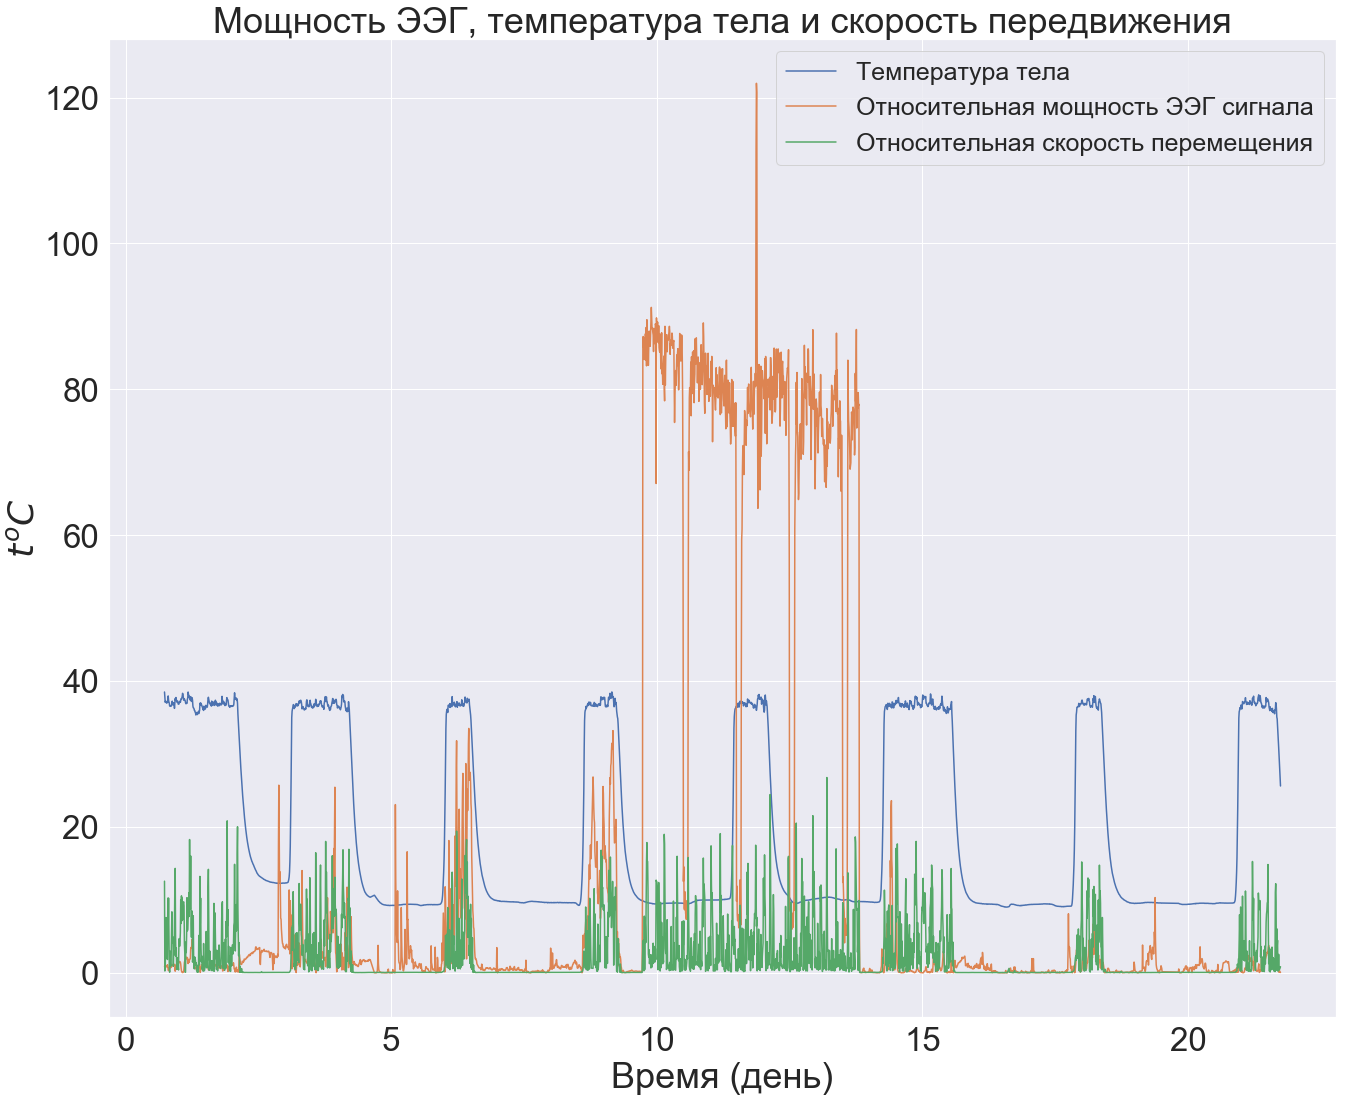
\includegraphics[width=\textwidth]{general.png}
  \captionof{figure}{Участок с большим содержанием артефактов не удален.}\label{fig:general}
\end{minipage}%
\begin{minipage}{.5\textwidth}
  \centering
  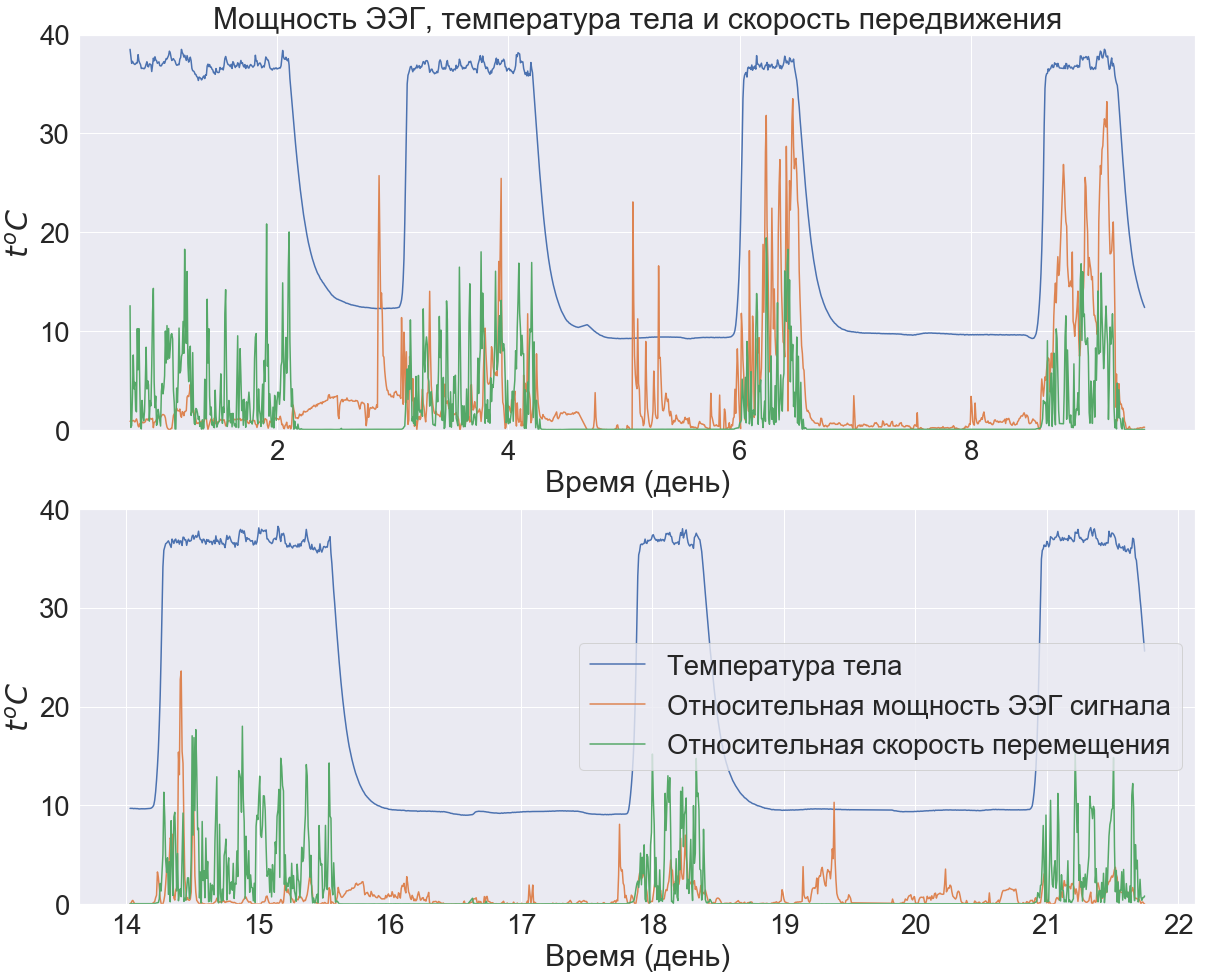
\includegraphics[width=\textwidth]{general2.png}
  \captionof{figure}{Участок с большим содержанием артефактов удален.}\label{fig:general2}
\end{minipage}
\end{figure}

Скорость на промежутке длинной $T$ может быть подсчитано по формуле $v_{x}(t_0, T) = \int_{t_0}^{t_0 + T} | a_{x}(t)| \; \text{d}t$. В случае физических сигналов средняя мощность на таком же промежутке подсчитывается по формуле $P(t_0, T) = \frac{1}{T} \int_{t_0}^{t_0 + T} [x(t)]^2 \; \text{d}t$. Для фильтрации был выбран КХИ-фильтр, потому что он устойчив, то есть поведение отфильтрованного сигнала «не сильно отличается» от поведения исходного сигнала. Это представляется важным, потому что артефакты, вызванные активностью, отличной от ЭЭГ, могут сильно привышать ЭЭГ по амплитуде и сильно исказить результат работы фильтров других типов.

В результате для каждой из записей были получены векторы значений скорости и мощности на 10-минутных временных интервалах, которые можно было сопоставить значениям термометра. Показания термометра, для которых не было соответствующих значений мощности и ускорения, были удалены из данных (\ref{fig:general}). В записи с 11 по 14 день наблюдается высокий всплеск мощности ЭЭГ и скорости перемещения животного. Такой сигнал сложно интерпретировать и, по всему видимому, он является продолжительным артефактом, который был удален из записи (\ref{fig:general2}, \ref{fig:general4},\ref{fig:general4}). 

\begin{figure}[H]
\centering
\begin{minipage}{.5\textwidth}
  \centering
  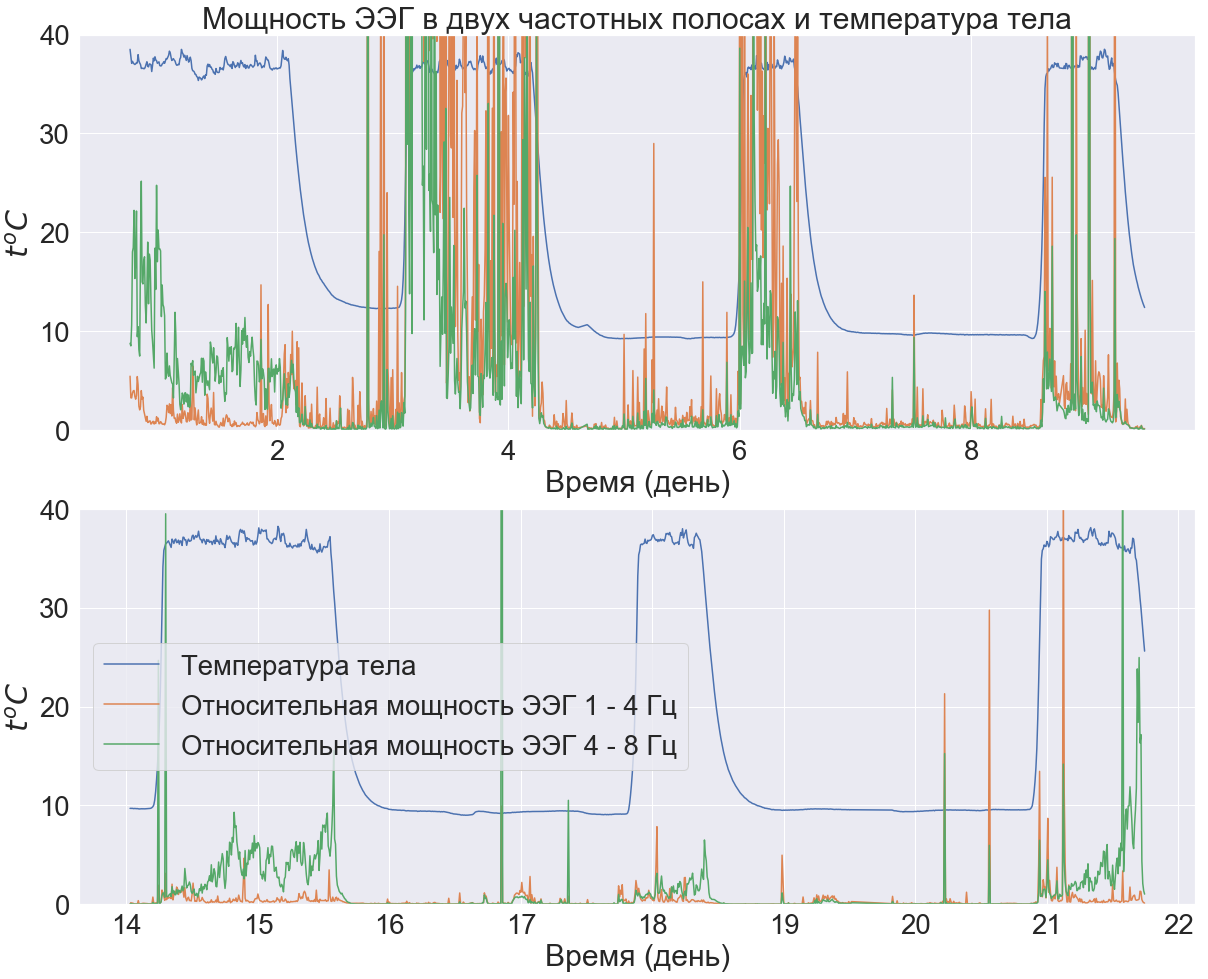
\includegraphics[width=\textwidth]{general3.png}
  \captionof{figure}{}\label{fig:general3}
\end{minipage}%
\begin{minipage}{.5\textwidth}
  \centering
  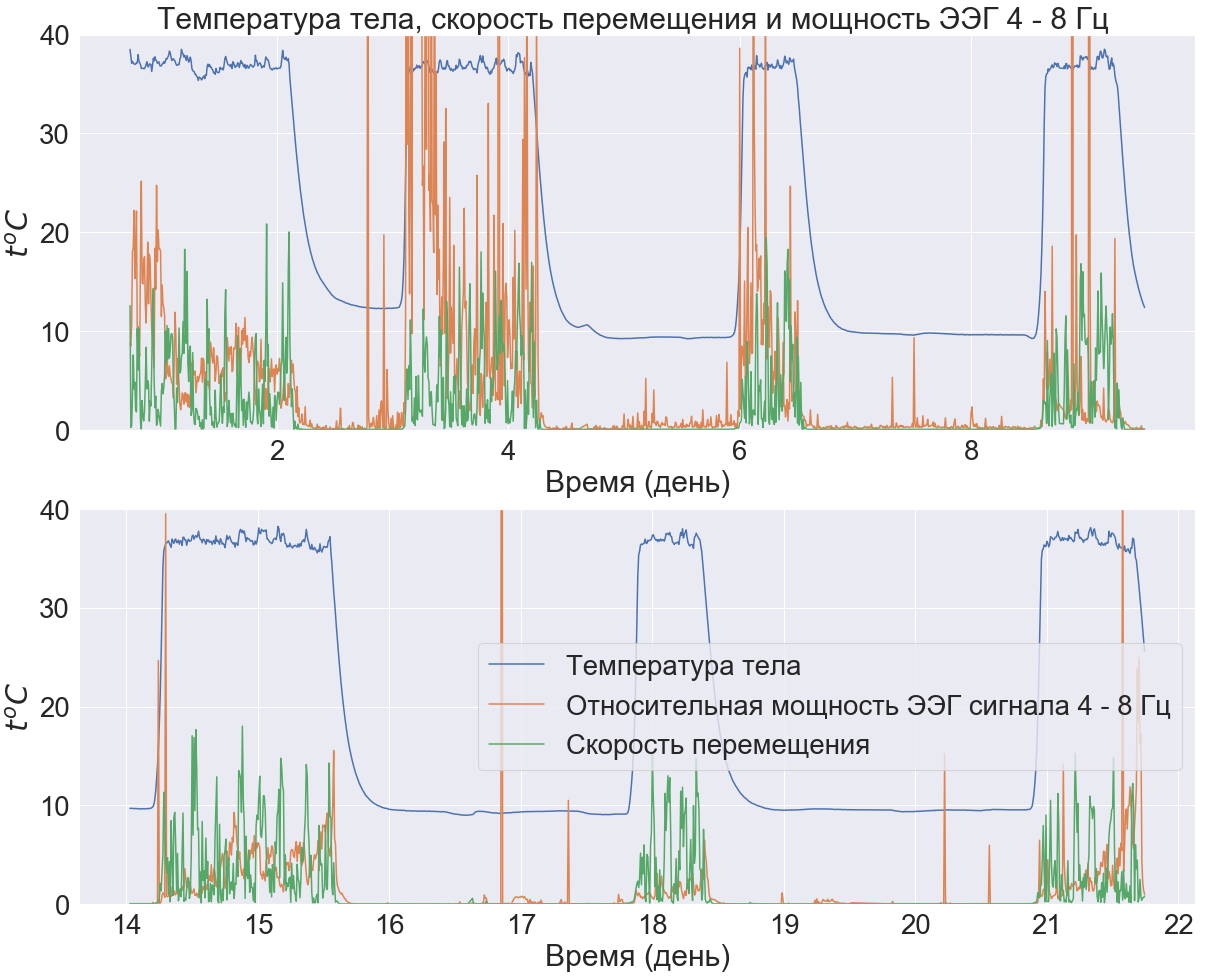
\includegraphics[width=\textwidth]{general4.png}
  \captionof{figure}{}\label{fig:general4}
\end{minipage}
\end{figure}

Судя по графикам, в первом промежутке выхода из торпора значения ЭЭГ были гораздо мощнее, чем при бодрствовании в самом начале эксперимента. Это может значить, что во время выхода из торпора затрата энергии начинается по всему телу для поднятия температуры, что влияет на ЭЭГ. При учете того, что в конце эксперимента хомяк погиб, можно предположить, что затрата энергии при выходе из торпора привела к истощению хомяка. 

\subsection{Статистика}

\begin{figure}[H]
\centering
\begin{minipage}{.5\textwidth}
  \centering
  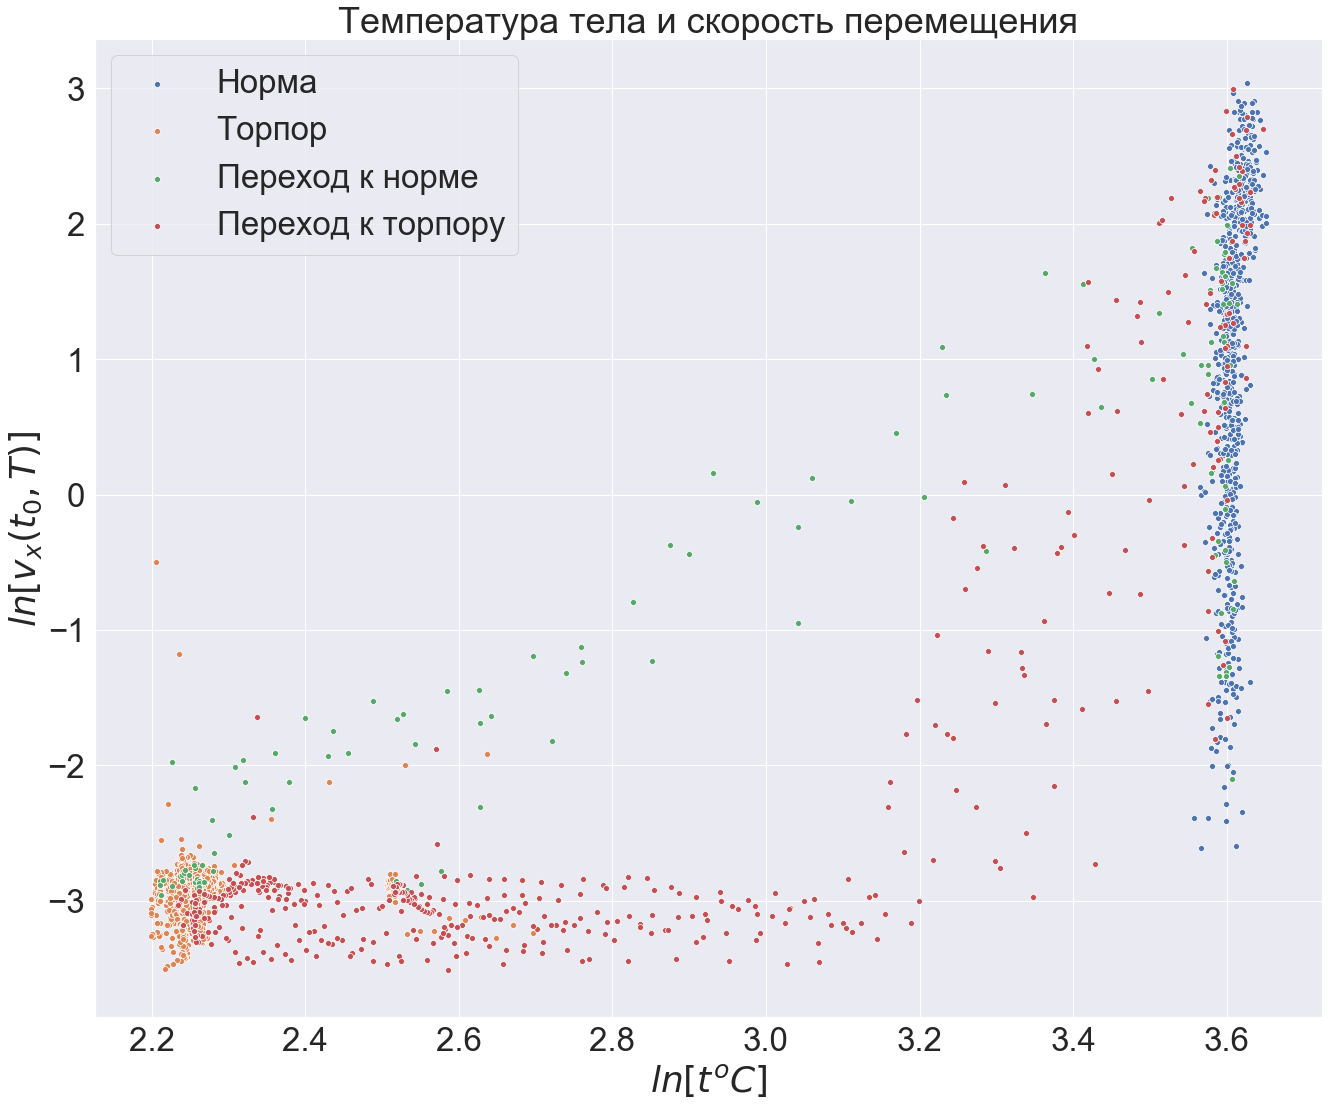
\includegraphics[width=\textwidth]{t_vs_speed.png}
  \captionof{figure}{}\label{fig:t_vs_speed}
\end{minipage}%
\begin{minipage}{.5\textwidth}
  \centering
  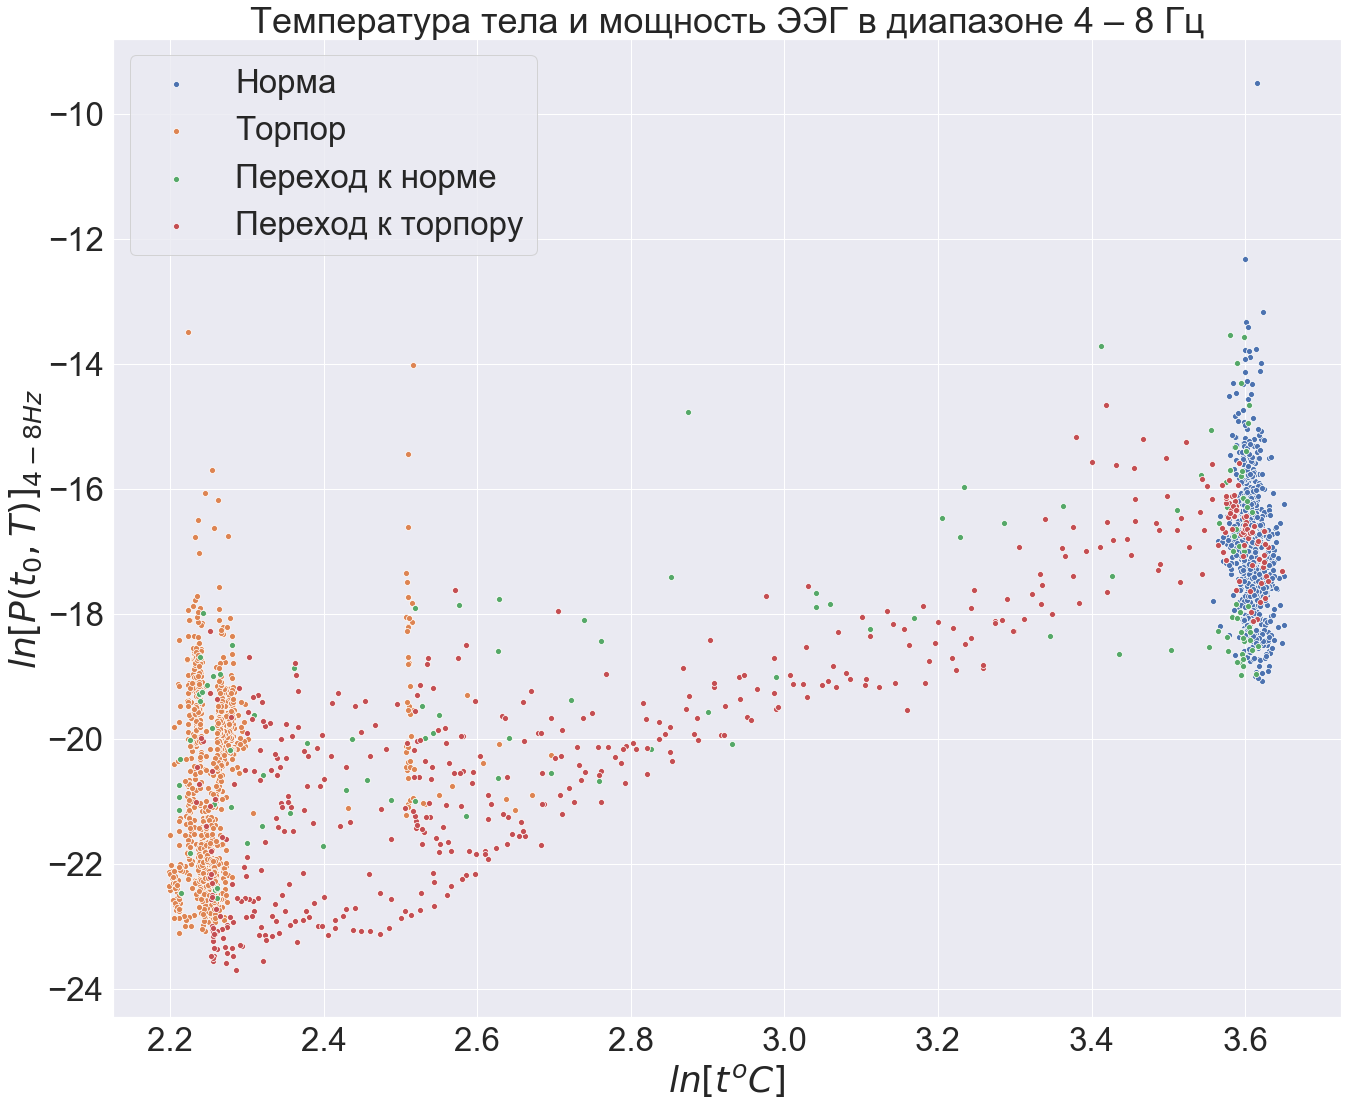
\includegraphics[width=\textwidth]{t_vs_p.png}
  \captionof{figure}{}\label{fig:t_vs_p}
\end{minipage}
\end{figure}

Диаграммы рассеяния позволяют выделить четыре состояния в которых мог находиться хомяк: норма, торпор, переход к торпору и переход к норме. 

Судя по диаграмме рассеяния для температуры тела хомяка и скорости его передвижения (\ref{fig:t_vs_speed}), скорость была ниже при низких температурах тела, что логично, потому что хомяк в этом случае впадал в торпор и не передвигался. При высоких температурах скорость наоборот была больше, потому что хомяк чаще бодрствовал и больше передвигался. При переходе от нормы к торпору видно, что раз хомяк останавливался и засыпал, а после этого у него начиналось понижение температуры тела. При переходе от торпора к норме видно, что скорость увеличивалась постепенно, а значит хомяк постепенно разогревался и был способен к более активному перемещению. 

Судя по диаграмме рассеяния для температуры тела хомяка и мощности ЭЭГ в диапозоне от 4 до 8 Гц (\ref{fig:t_vs_p}), мощность была ниже при низких температурах тела, что в состоянии торпора хомяк экономит энергию. При высоких температурах мощность наоборот была больше, потому что хомяк бодрствовал и его мозг расходовал энергию, что приводило к электрической активности клеток. Однако, в отличии от скорости, мощность постепенно росла или убывала при выходе или входе в состояние торпора соответственно. 

\begin{figure}[H]
\centering
\begin{minipage}{.5\textwidth}
  \centering
  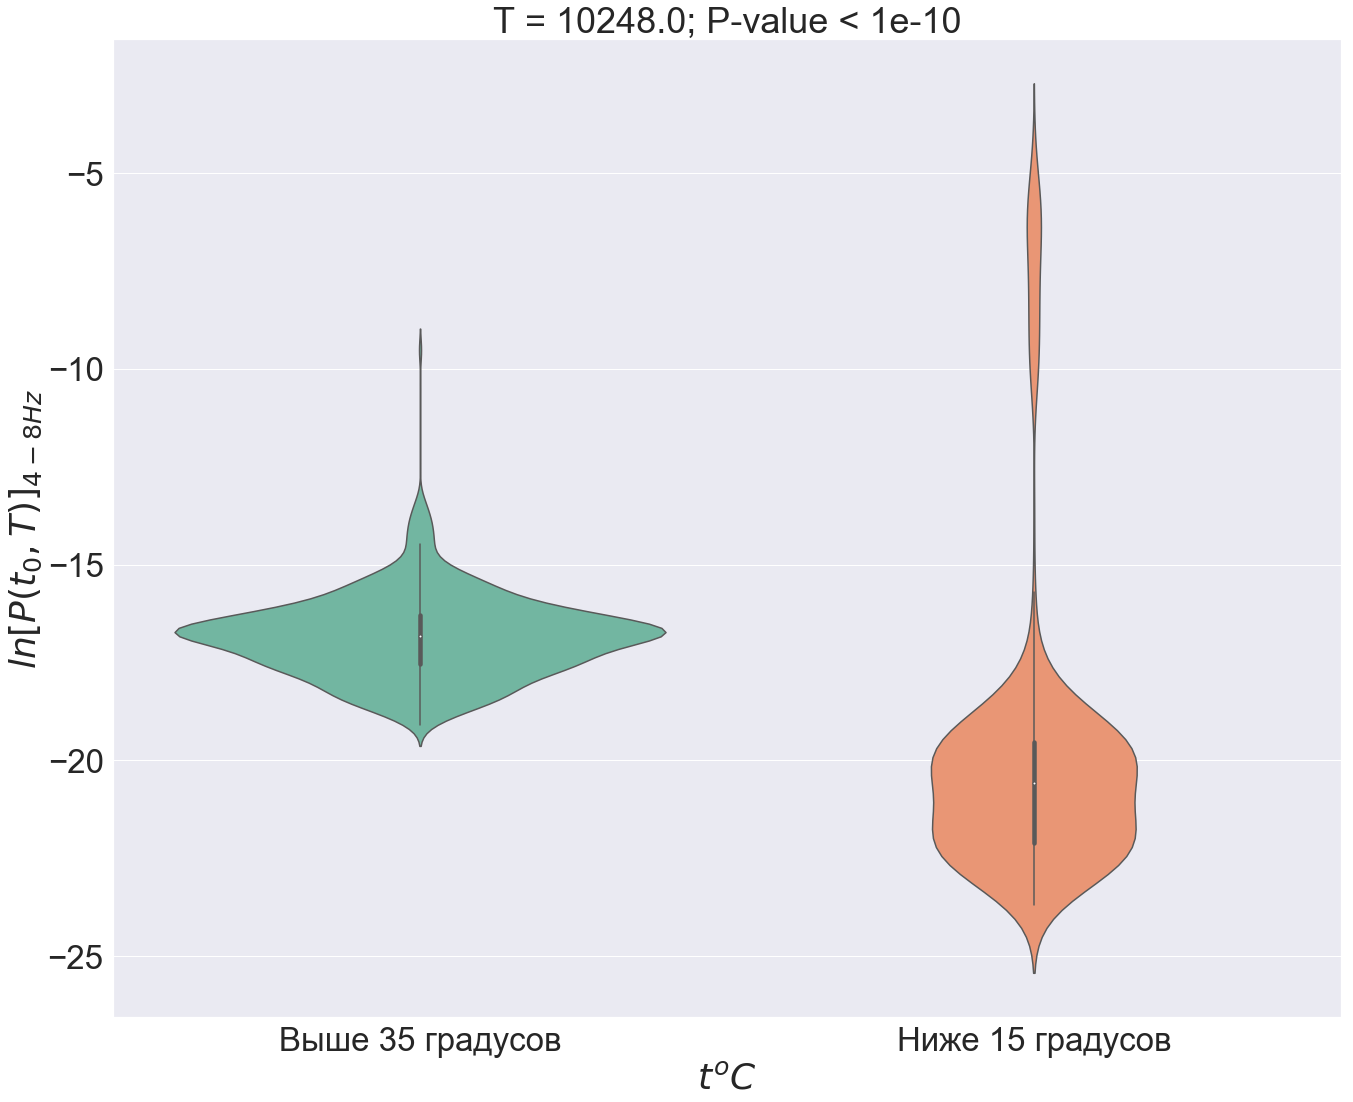
\includegraphics[width=\textwidth]{violin_plot1.png}
  \captionof{figure}{}\label{fig:violin_plot1}
\end{minipage}%
\begin{minipage}{.5\textwidth}
  \centering
  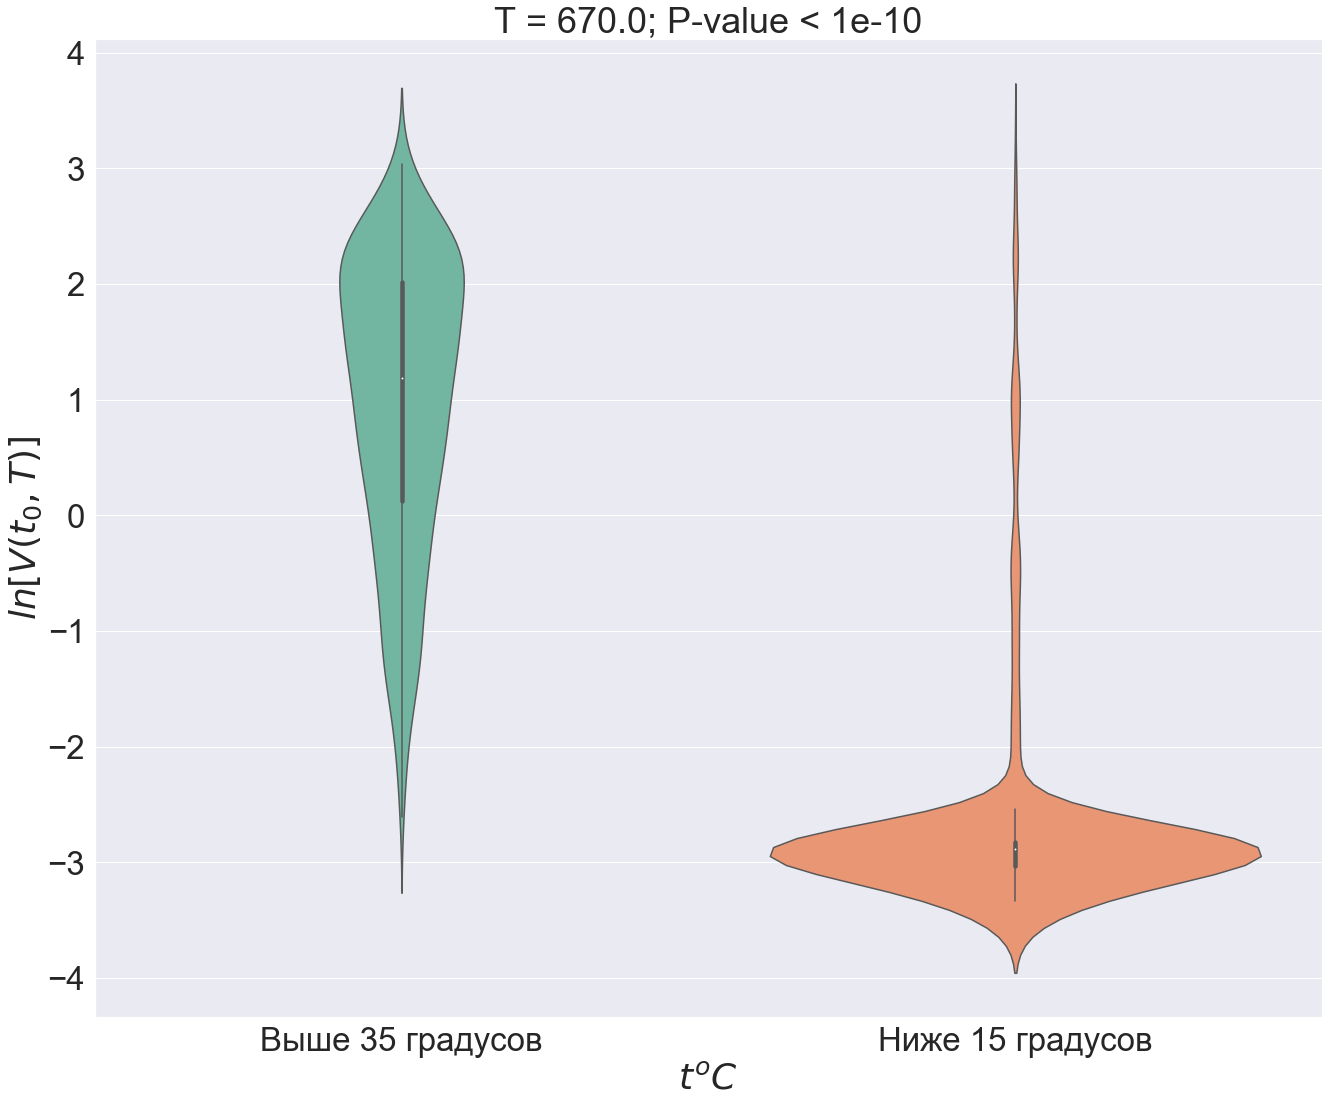
\includegraphics[width=\textwidth]{violin_plot2.png}
  \captionof{figure}{}\label{fig:violin_plot2}
\end{minipage}
\end{figure}

В зависимости от того, в каком состоянии находился хомяк, торпора или бодрствования, различия оказались значимы и между скоростью передвижения хомяка ($T = 9435$, $p < 10^{-10}$)(\ref{fig:violin_plot1}), и между мощностью ЭЭГ-сигнала в частотной полосе от 4 до 8 Гц ($T = 620$, $p < 10^{-10}$) (\ref{fig:violin_plot2}). 

\begin{figure}[H]
\centering
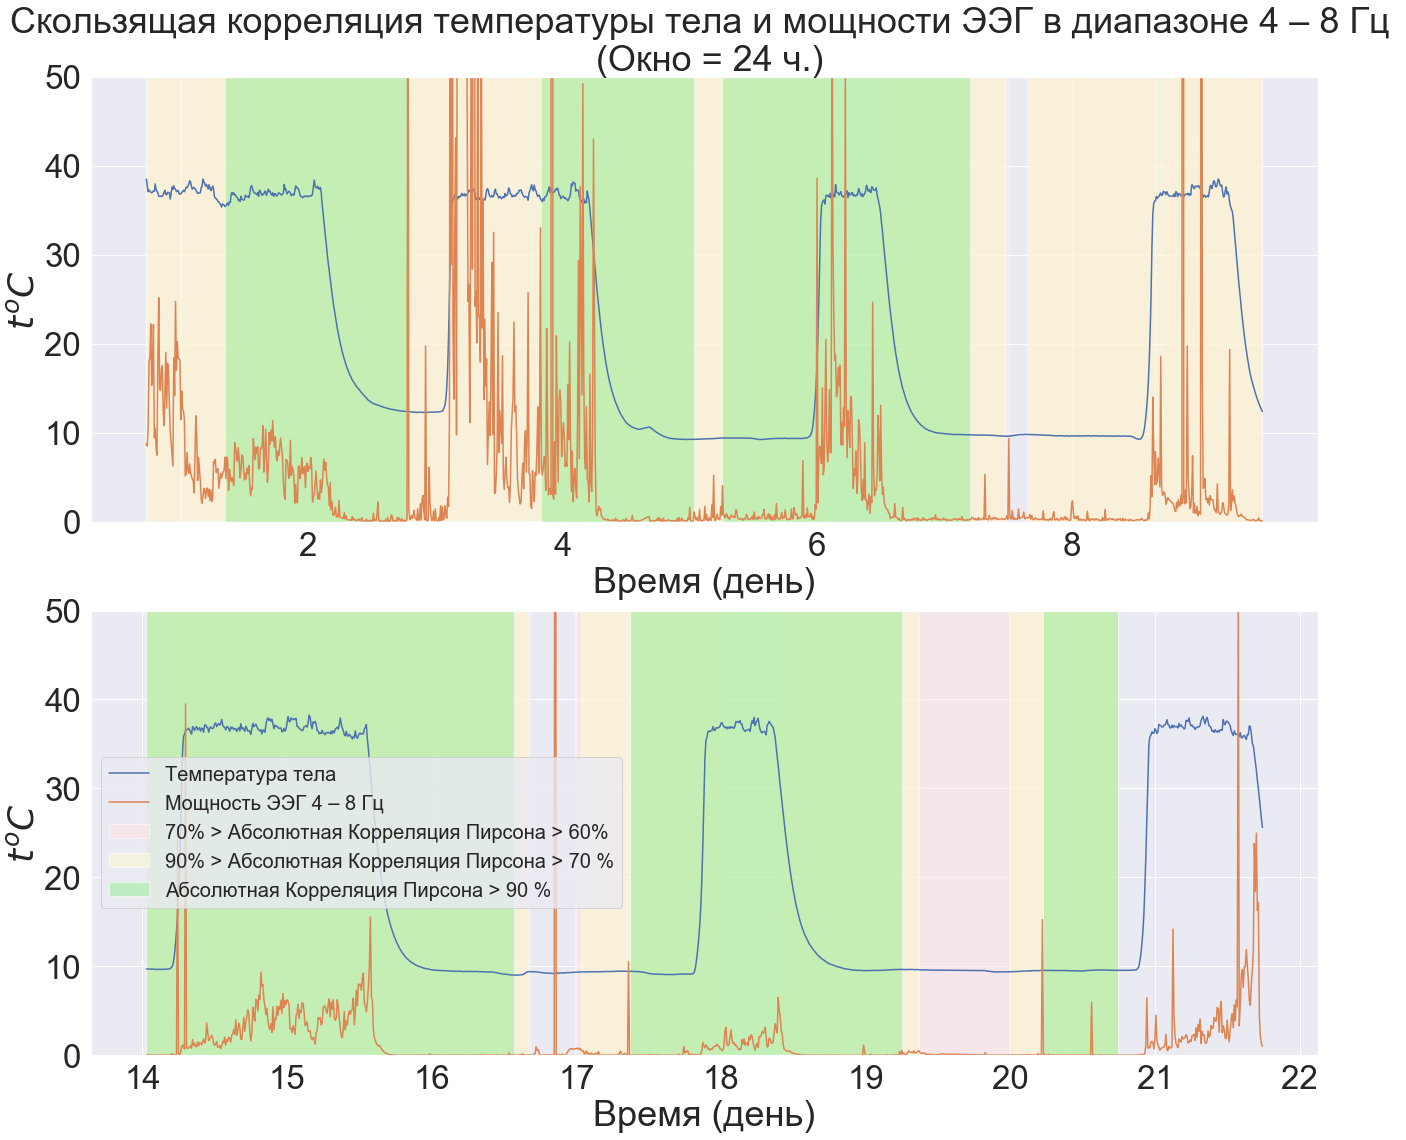
\includegraphics[width=0.7\linewidth]{moving_correlation.png}
\caption{}\label{fig:moving_correlation}
\end{figure}

Метод скользящего окна для корреляции Пирсона позволил установить наличие значимой корреляции логарифмированной мощности и температуры тела на разных временных интервалах проведенного эксперимента. Подробный результат представлен на рисунке \ref{fig:moving_correlation}.


% \begin{figure}
%   \centering
%   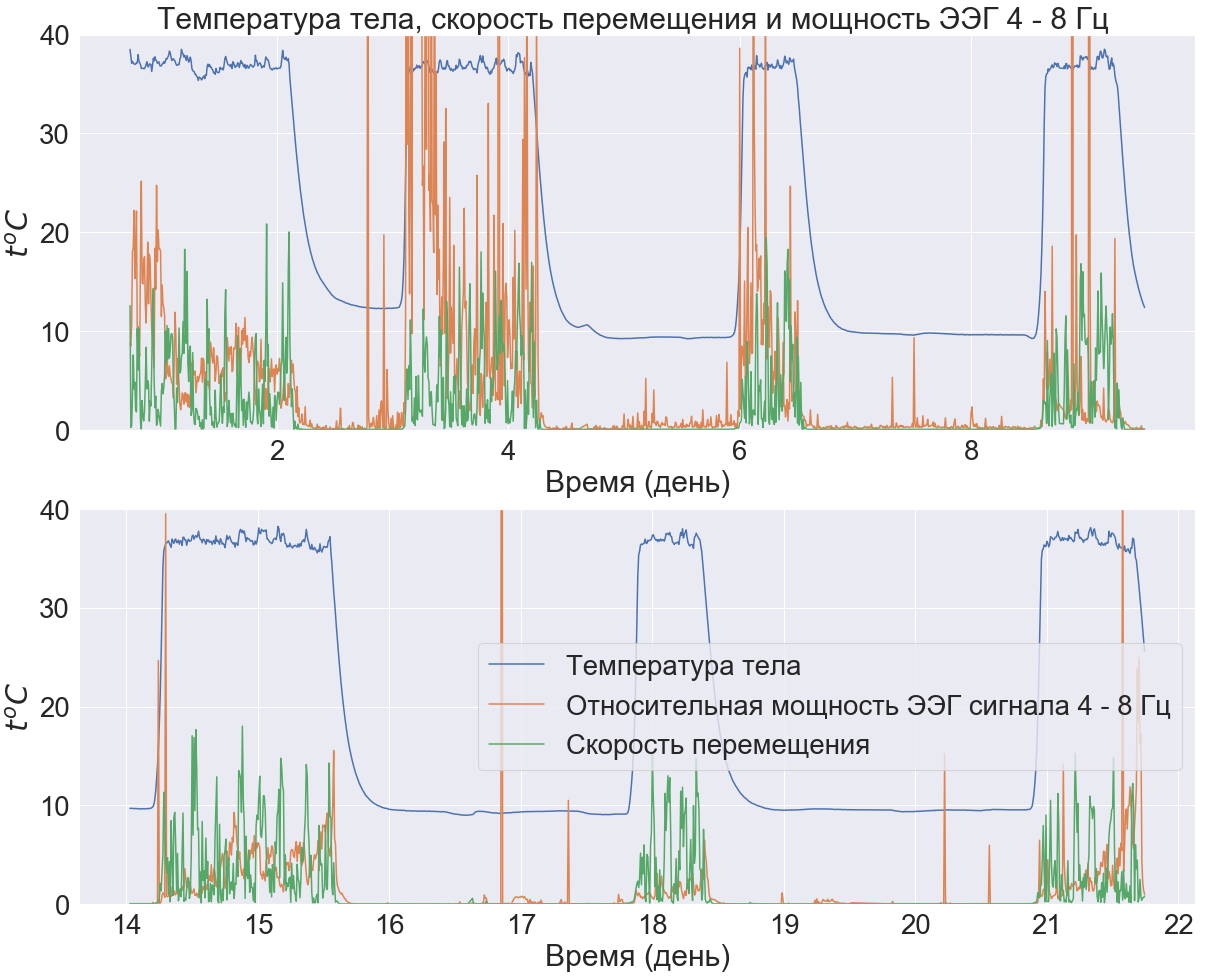
\includegraphics[width=\textwidth]{general4.png}
%   \caption{}
%   \label{fig:general4}
% \end{figure}

% \begin{figure}
%   \centering
%   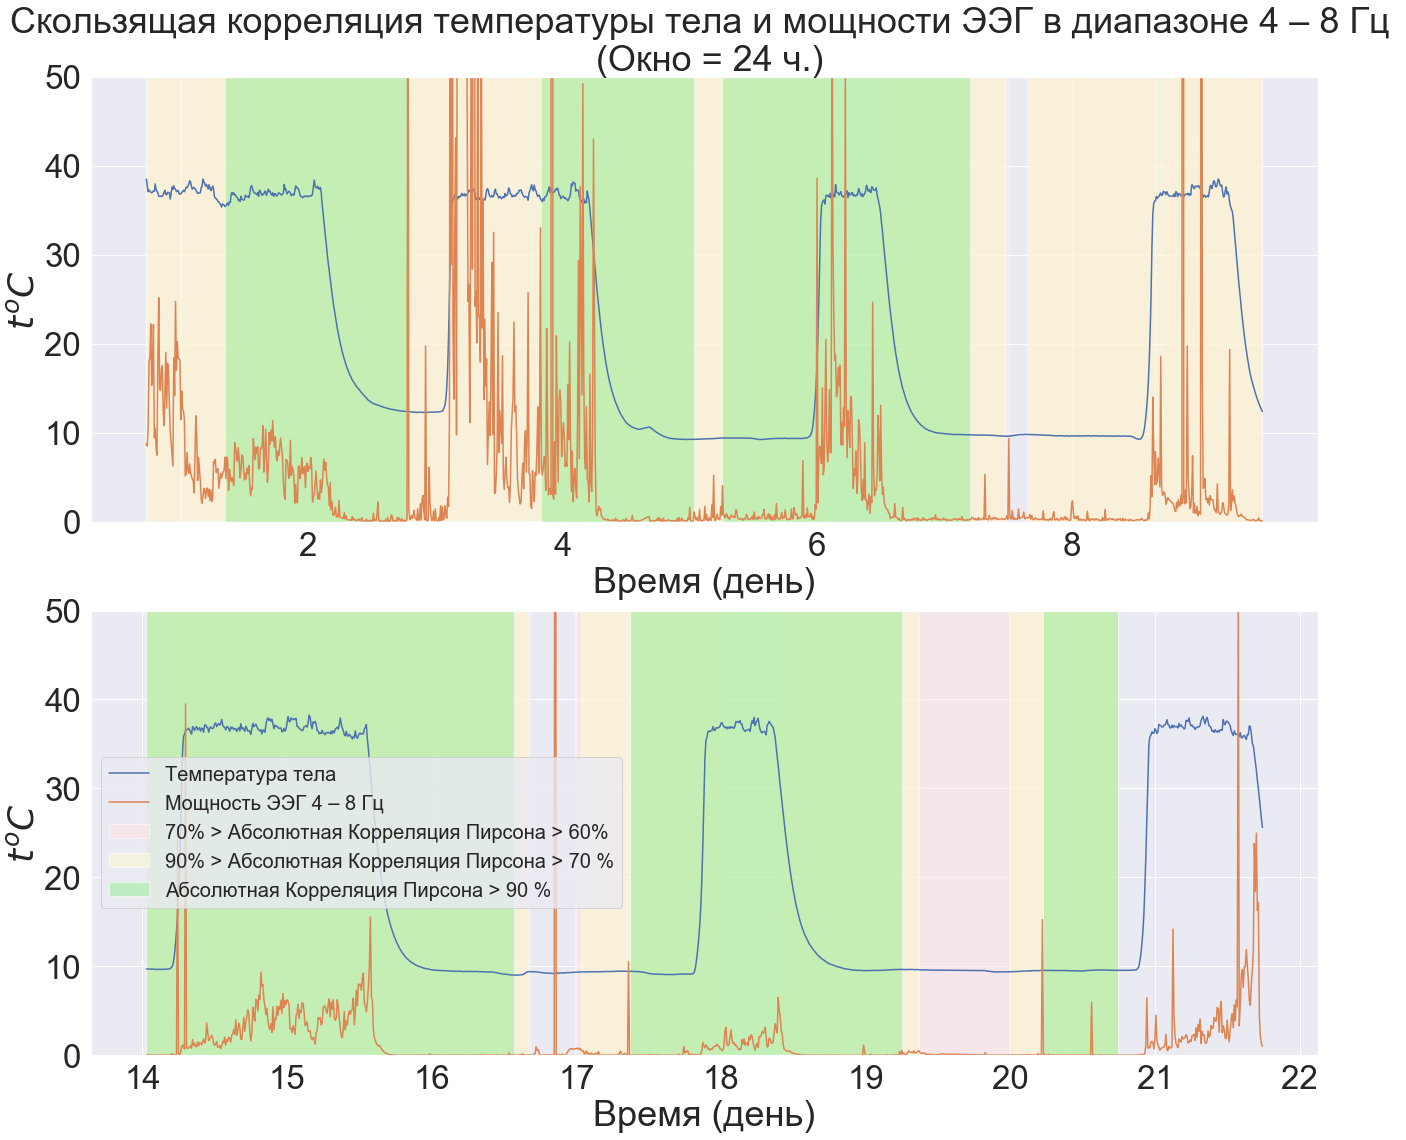
\includegraphics[width=\textwidth]{moving_correlation.png}
%   \caption{}
%   \label{fig:moving_correlation}
% \end{figure}

% \begin{figure}
%   \centering
%   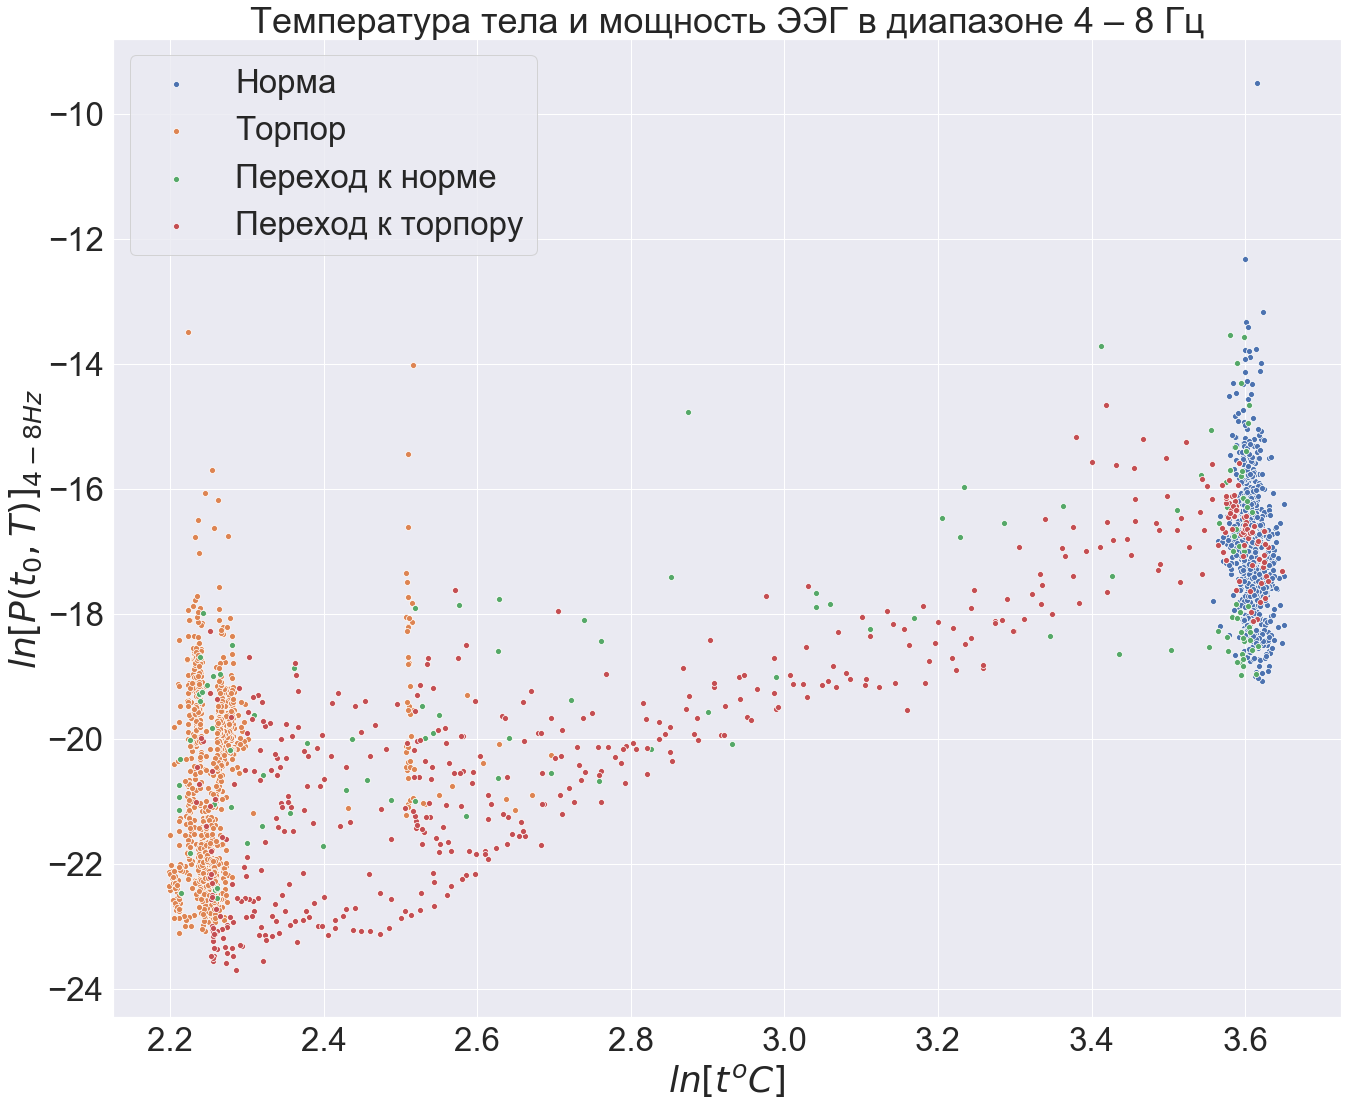
\includegraphics[width=\textwidth]{t_vs_p.png}
%   \caption{}
%   \label{fig:t_vs_p}
% \end{figure}

% \begin{figure}
%   \centering
%   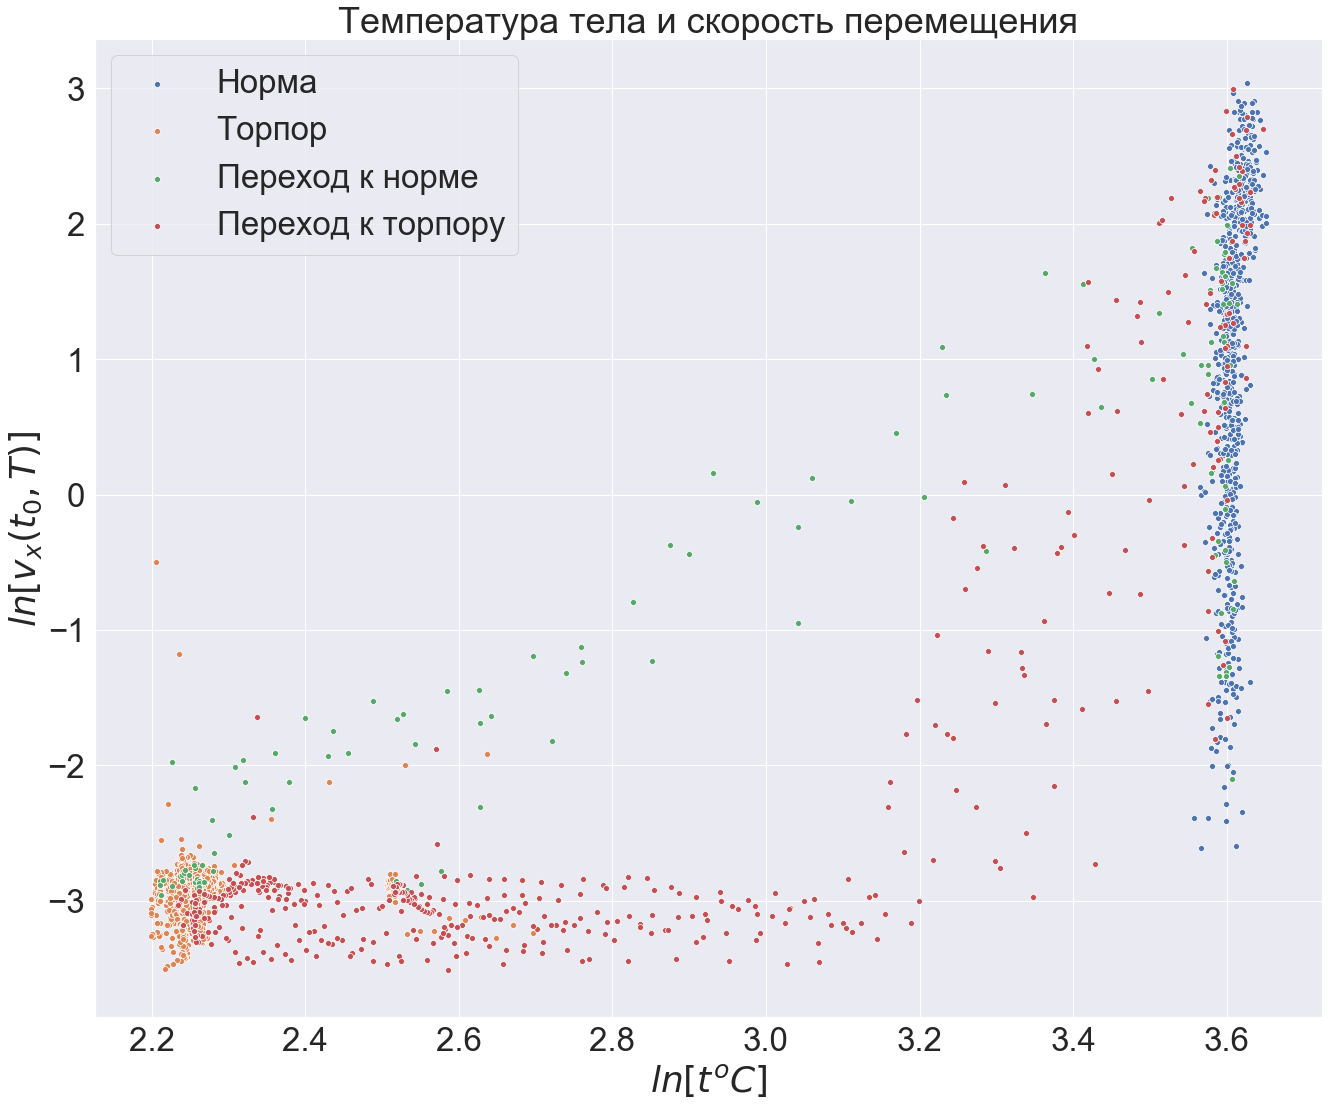
\includegraphics[width=\textwidth]{t_vs_speed.png}
%   \caption{}
%   \label{fig:t_vs_speed}
% \end{figure}

% \begin{figure}
%   \centering
%   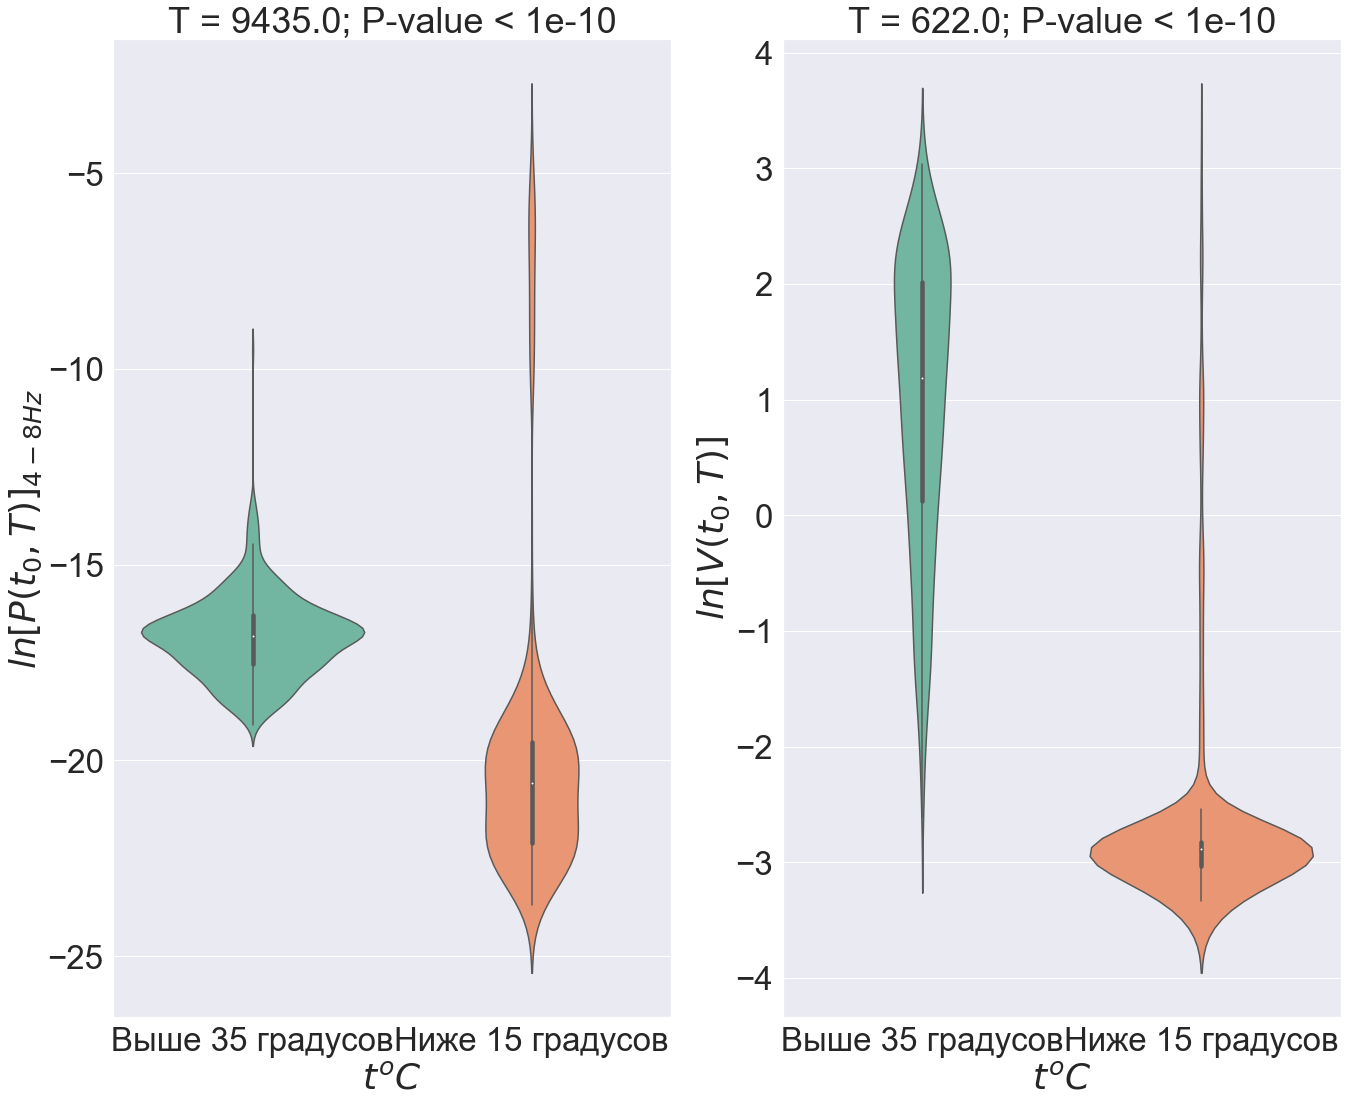
\includegraphics[width=\textwidth]{violin_plot.png}
%   \caption{}
%   \label{fig:violin_plot}
% \end{figure}

\section{Приложение}

Код, выполняющий все вычисления, может быть найден \href{https://github.com/BasilMinkov/Jupyter-Notebooks/blob/master/HamsterEEG.ipynb}{в моем репозитории GitHub}. Код написан в \textbf{Jupyter Notebook} на языке \textbf{Python 3}.


\bibliographystyle{apalike}
\bibliography{/Users/wassilyminkow/Scripts/LaTeX/library.bib}

% \begin{info} % Information block
% 	This is an interesting piece of information, to which the reader should pay special attention. Fusce varius orci ac magna dapibus porttitor. In tempor leo a neque bibendum sollicitudin. Nulla pretium fermentum nisi, eget sodales magna facilisis eu. Praesent aliquet nulla ut bibendum lacinia. Donec vel mauris vulputate, commodo ligula ut, egestas orci. Suspendisse commodo odio sed hendrerit lobortis. Donec finibus eros erat, vel ornare enim mattis et.
% \end{info}

% %----------------------------------------------------------------------------------------
% %	PROBLEM 1
% %----------------------------------------------------------------------------------------

% \section{Problem title} % Numbered section

% In hac habitasse platea dictumst. Curabitur mattis elit sit amet justo luctus vestibulum. In hac habitasse platea dictumst. Pellentesque lobortis justo enim, a condimentum massa tempor eu. Ut quis nulla a quam pretium eleifend nec eu nisl. Nam cursus porttitor eros, sed luctus ligula convallis quis. Nam convallis, ligula in auctor euismod, ligula mauris fringilla tellus, et egestas mauris odio eget diam. Praesent sodales in ipsum eu dictum.

% %------------------------------------------------

% \subsection{Theoretical viewpoint}

% Maecenas consectetur metus at tellus finibus condimentum. Proin arcu lectus, ultrices non tincidunt et, tincidunt ut quam. Integer luctus posuere est, non maximus ante dignissim quis. Nunc a cursus erat. Curabitur suscipit nibh in tincidunt sagittis. Nam malesuada vestibulum quam id gravida. Proin ut dapibus velit. Vestibulum eget quam quis ipsum semper convallis. Duis consectetur nibh ac diam dignissim, id condimentum enim dictum. Nam aliquet ligula eu magna pellentesque, nec sagittis leo lobortis. Aenean tincidunt dignissim egestas. Morbi efficitur risus ante, id tincidunt odio pulvinar vitae.

% Curabitur tempus hendrerit nulla. Donec faucibus lobortis nibh pharetra sagittis. Sed magna sem, posuere eget sem vitae, finibus consequat libero. Cras aliquet sagittis erat ut semper. Aenean vel enim ipsum. Fusce ut felis at eros sagittis bibendum mollis lobortis libero. Donec laoreet nisl vel risus lacinia elementum non nec lacus. Nullam luctus, nulla volutpat ultricies ultrices, quam massa placerat augue, ut fringilla urna lectus nec nibh. Vestibulum efficitur condimentum orci a semper. Pellentesque ut metus pretium lacus maximus semper. Sed tellus augue, consectetur rhoncus eleifend vel, imperdiet nec turpis. Nulla ligula ante, malesuada quis orci a, ultricies blandit elit.

% % Numbered question, with subquestions in an enumerate environment
% \begin{question}
% 	Quisque ullamcorper placerat ipsum. Cras nibh. Morbi vel justo vitae lacus tincidunt ultrices. Lorem ipsum dolor sit amet, consectetuer adipiscing elit.

% 	% Subquestions numbered with letters
% 	\begin{enumerate}[(a)]
% 		\item Do this.
% 		\item Do that.
% 		\item Do something else.
% 	\end{enumerate}
% \end{question}
	
% %------------------------------------------------

% \subsection{Algorithmic issues}

% In malesuada ullamcorper urna, sed dapibus diam sollicitudin non. Donec elit odio, accumsan ac nisl a, tempor imperdiet eros. Donec porta tortor eu risus consequat, a pharetra tortor tristique. Morbi sit amet laoreet erat. Morbi et luctus diam, quis porta ipsum. Quisque libero dolor, suscipit id facilisis eget, sodales volutpat dolor. Nullam vulputate interdum aliquam. Mauris id convallis erat, ut vehicula neque. Sed auctor nibh et elit fringilla, nec ultricies dui sollicitudin. Vestibulum vestibulum luctus metus venenatis facilisis. Suspendisse iaculis augue at vehicula ornare. Sed vel eros ut velit fermentum porttitor sed sed massa. Fusce venenatis, metus a rutrum sagittis, enim ex maximus velit, id semper nisi velit eu purus.

% \begin{center}
% 	\begin{minipage}{0.5\linewidth} % Adjust the minipage width to accomodate for the length of algorithm lines
% 		\begin{algorithm}[H]
% 			\KwIn{$(a, b)$, two floating-point numbers}  % Algorithm inputs
% 			\KwResult{$(c, d)$, such that $a+b = c + d$} % Algorithm outputs/results
% 			\medskip
% 			\If{$\vert b\vert > \vert a\vert$}{
% 				exchange $a$ and $b$ \;
% 			}
% 			$c \leftarrow a + b$ \;
% 			$z \leftarrow c - a$ \;
% 			$d \leftarrow b - z$ \;
% 			{\bf return} $(c,d)$ \;
% 			\caption{\texttt{FastTwoSum}} % Algorithm name
% 			\label{alg:fastTwoSum}   % optional label to refer to
% 		\end{algorithm}
% 	\end{minipage}
% \end{center}

% Fusce varius orci ac magna dapibus porttitor. In tempor leo a neque bibendum sollicitudin. Nulla pretium fermentum nisi, eget sodales magna facilisis eu. Praesent aliquet nulla ut bibendum lacinia. Donec vel mauris vulputate, commodo ligula ut, egestas orci. Suspendisse commodo odio sed hendrerit lobortis. Donec finibus eros erat, vel ornare enim mattis et.

% % Numbered question, with an optional title
% \begin{question}[\itshape (with optional title)]
% 	In congue risus leo, in gravida enim viverra id. Donec eros mauris, bibendum vel dui at, tempor commodo augue. In vel lobortis lacus. Nam ornare ullamcorper mauris vel molestie. Maecenas vehicula ornare turpis, vitae fringilla orci consectetur vel. Nam pulvinar justo nec neque egestas tristique. Donec ac dolor at libero congue varius sed vitae lectus. Donec et tristique nulla, sit amet scelerisque orci. Maecenas a vestibulum lectus, vitae gravida nulla. Proin eget volutpat orci. Morbi eu aliquet turpis. Vivamus molestie urna quis tempor tristique. Proin hendrerit sem nec tempor sollicitudin.
% \end{question}

% Mauris interdum porttitor fringilla. Proin tincidunt sodales leo at ornare. Donec tempus magna non mauris gravida luctus. Cras vitae arcu vitae mauris eleifend scelerisque. Nam sem sapien, vulputate nec felis eu, blandit convallis risus. Pellentesque sollicitudin venenatis tincidunt. In et ipsum libero. Nullam tempor ligula a massa convallis pellentesque.

% %----------------------------------------------------------------------------------------
% %	PROBLEM 2
% %----------------------------------------------------------------------------------------

% \section{Implementation}

% Proin lobortis efficitur dictum. Pellentesque vitae pharetra eros, quis dignissim magna. Sed tellus leo, semper non vestibulum vel, tincidunt eu mi. Aenean pretium ut velit sed facilisis. Ut placerat urna facilisis dolor suscipit vehicula. Ut ut auctor nunc. Nulla non massa eros. Proin rhoncus arcu odio, eu lobortis metus sollicitudin eu. Duis maximus ex dui, id bibendum diam dignissim id. Aliquam quis lorem lorem. Phasellus sagittis aliquet dolor, vulputate cursus dolor convallis vel. Suspendisse eu tellus feugiat, bibendum lectus quis, fermentum nunc. Nunc euismod condimentum magna nec bibendum. Curabitur elementum nibh eu sem cursus, eu aliquam leo rutrum. Sed bibendum augue sit amet pharetra ullamcorper. Aenean congue sit amet tortor vitae feugiat.

% In congue risus leo, in gravida enim viverra id. Donec eros mauris, bibendum vel dui at, tempor commodo augue. In vel lobortis lacus. Nam ornare ullamcorper mauris vel molestie. Maecenas vehicula ornare turpis, vitae fringilla orci consectetur vel. Nam pulvinar justo nec neque egestas tristique. Donec ac dolor at libero congue varius sed vitae lectus. Donec et tristique nulla, sit amet scelerisque orci. Maecenas a vestibulum lectus, vitae gravida nulla. Proin eget volutpat orci. Morbi eu aliquet turpis. Vivamus molestie urna quis tempor tristique. Proin hendrerit sem nec tempor sollicitudin.

% % File contents
% \begin{file}[hello.py]
% \begin{lstlisting}[language=Python]
% #! /usr/bin/python

% import sys
% sys.stdout.write("Hello World!\n")
% \end{lstlisting}
% \end{file}

% Fusce eleifend porttitor arcu, id accumsan elit pharetra eget. Mauris luctus velit sit amet est sodales rhoncus. Donec cursus suscipit justo, sed tristique ipsum fermentum nec. Ut tortor ex, ullamcorper varius congue in, efficitur a tellus. Vivamus ut rutrum nisi. Phasellus sit amet enim efficitur, aliquam nulla id, lacinia mauris. Quisque viverra libero ac magna maximus efficitur. Interdum et malesuada fames ac ante ipsum primis in faucibus. Vestibulum mollis eros in tellus fermentum, vitae tristique justo finibus. Sed quis vehicula nibh. Etiam nulla justo, pellentesque id sapien at, semper aliquam arcu. Integer at commodo arcu. Quisque dapibus ut lacus eget vulputate.

% % Command-line "screenshot"
% \begin{commandline}
% 	\begin{verbatim}
% 		$ chmod +x hello.py
% 		$ ./hello.py

% 		Hello World!
% 	\end{verbatim}
% \end{commandline}

% Vestibulum sodales orci a nisi interdum tristique. In dictum vehicula dui, eget bibendum purus elementum eu. Pellentesque lobortis mattis mauris, non feugiat dolor vulputate a. Cras porttitor dapibus lacus at pulvinar. Praesent eu nunc et libero porttitor malesuada tempus quis massa. Aenean cursus ipsum a velit ultricies sagittis. Sed non leo ullamcorper, suscipit massa ut, pulvinar erat. Aliquam erat volutpat. Nulla non lacus vitae mi placerat tincidunt et ac diam. Aliquam tincidunt augue sem, ut vestibulum est volutpat eget. Suspendisse potenti. Integer condimentum, risus nec maximus elementum, lacus purus porta arcu, at ultrices diam nisl eget urna. Curabitur sollicitudin diam quis sollicitudin varius. Ut porta erat ornare laoreet euismod. In tincidunt purus dui, nec egestas dui convallis non. In vestibulum ipsum in dictum scelerisque.

% % Warning text, with a custom title
% \begin{warn}[Notice:]
%   In congue risus leo, in gravida enim viverra id. Donec eros mauris, bibendum vel dui at, tempor commodo augue. In vel lobortis lacus. Nam ornare ullamcorper mauris vel molestie. Maecenas vehicula ornare turpis, vitae fringilla orci consectetur vel. Nam pulvinar justo nec neque egestas tristique. Donec ac dolor at libero congue varius sed vitae lectus. Donec et tristique nulla, sit amet scelerisque orci. Maecenas a vestibulum lectus, vitae gravida nulla. Proin eget volutpat orci. Morbi eu aliquet turpis. Vivamus molestie urna quis tempor tristique. Proin hendrerit sem nec tempor sollicitudin.
% \end{warn}

%----------------------------------------------------------------------------------------

\end{document}
